% alt: Two panels. Left, a chain of five blocks B_1 to B_5 on a line with a sweep party graph above it in blue: block owners P_1 to P_5 in a row above their blocks, remainders R_0 to R_4 in a higher row with R_k above block k+1, and the links of each step joining P_k, P_{k+1}, R_k and R_{k+1}; an orange dashed line through the bond between B_2 and B_3 is crossed by three links and reads "O(1) links cross". Right, a complete binary tree of dyadic intervals over a line of eight sites, each interval a grey bar with its party dot at the first site of its right half, grey links from each party to its two children; an orange dashed line through the bond between sites 3 and 4 is crossed by one link at every level and reads "log L links cross: cutwidth log L".
% Section 12 (Assembly on the chain), the placement in the proof of Theorem thm:B (attach P_i to block B_i and R_k to block B_{k+1}; a bond between blocks is crossed only by links among the parties attached to the nearest blocks, at most chi links), and the remark at the end of Section 10 (The sweep) on why a sweep rather than the dyadic hierarchy of the source (every scale has a link crossing a bond, cutwidth log L) (part2b_mps_protocol.tex). Left panel: the line is the chain Lambda cut into the blocks B_i of Construction con:sweep, continued to the right by dots; each blue dot is one party of the sweep, P_i attached to B_i and R_k attached to B_{k+1}; each blue link joins two parties that share a gate at step k of Construction con:sweep, namely R_k-R_{k+1} (move (1)), P_{k+1}-R_k (move (2) and the band dissolutions), P_k-R_k and P_k-P_{k+1} (move (3), the band between C = P_k and B = P_{k+1}), P_{k+1}-R_{k+1} (move (4), the band between C = P_{k+1} and B = R_{k+1}); the two links leaving the picture at the right go to R_5; the orange dashed line is the block bond B_2 | B_3 and the three links crossing it are R_1-R_2, P_2-P_3 and P_2-R_2. Right panel: the sites are the leaves, each grey bar is a dyadic interval of length 2, 4 and 8 = L, its dot is the party of that interval drawn at the first site of its right half, and each grey link joins an interval to one of its two halves; the orange dashed line is the bond 3 | 4 and the three links crossing it, one per level, are [1,8]-[1,4], [1,4]-[3,4] and [3,4]-{3}. No tensor is drawn and no leg is contracted; the links are the links of the party network, not legs.
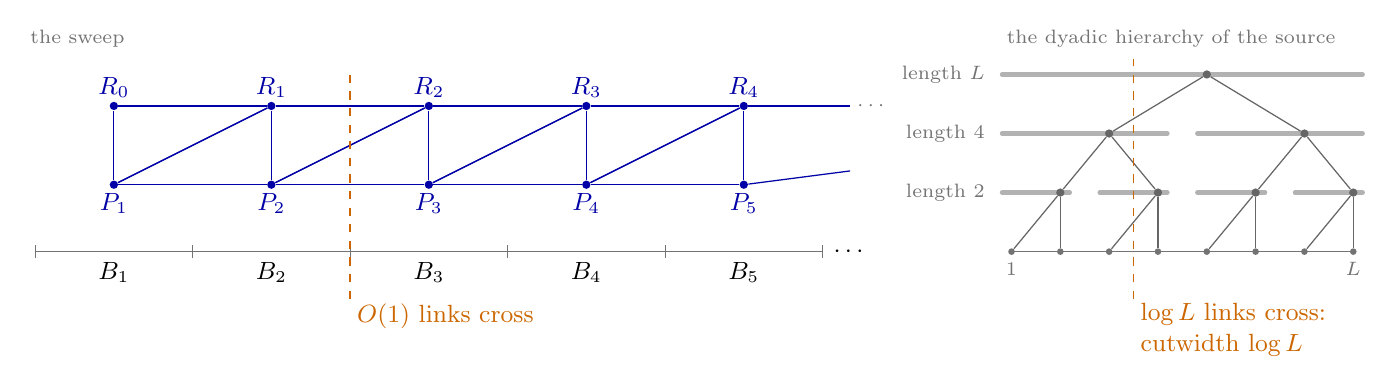
\begin{tikzpicture}[x=1cm, y=1cm, line width=0.3pt,
    lab/.style={font=\small, inner sep=1pt},
    annot/.style={font=\scriptsize, text=black!55, inner sep=1pt},
    party/.style={circle, fill=blue!65!black, inner sep=0pt, minimum size=3pt},
    link/.style={draw=blue!65!black, line width=0.45pt},
    site/.style={circle, fill=black!55, inner sep=0pt, minimum size=2.4pt},
    dnode/.style={circle, fill=black!60, inner sep=0pt, minimum size=3pt},
    dlink/.style={draw=black!60, line width=0.45pt},
    bar/.style={draw=black!30, line width=1.6pt, line cap=round},
    cut/.style={dashed, color=orange!80!black, line width=0.5pt}]
  % ================= left panel: the sweep party graph on the chain ========
  % geometry: blocks of width \b on the chain line y = 0, block owners P_i at
  % height \yP above the centre of B_i, remainders R_k at height \yR above the
  % centre of B_{k+1}; the chain continues to the right (dots)
  \def\b{2.0}\def\yP{0.85}\def\yR{1.85}
  \node[annot, anchor=south west] at (-0.1, 2.55) {the sweep};
  % the chain and its blocks
  \draw[black!55] (0, 0) -- (5*\b, 0);
  \foreach \i in {0,...,5} { \draw[black!55] (\i*\b, 0.08) -- (\i*\b, -0.08); }
  \foreach \i in {1,...,5} {
    \node[lab, anchor=north] at ({(\i-0.5)*\b}, -0.1) {\(B_{\i}\)};
  }
  \node[lab, anchor=west] at (5*\b + 0.1, 0) {\(\cdots\)};
  % parties: P_i above B_i, R_k above B_{k+1}
  \foreach \i in {1,...,5} {
    \node[party] (P\i) at ({(\i-0.5)*\b}, \yP) {};
    \node[lab, anchor=north, text=blue!65!black] at ({(\i-0.5)*\b}, \yP-0.07) {\(P_{\i}\)};
  }
  \foreach \k in {0,...,4} {
    \pgfmathtruncatemacro{\j}{\k+1}
    \node[party] (R\k) at ({(\j-0.5)*\b}, \yR) {};
    \node[lab, anchor=south, text=blue!65!black] at ({(\j-0.5)*\b}, \yR+0.07) {\(R_{\k}\)};
  }
  % links of step k = 0: the band of block 1 dies into P_1
  \draw[link] (P1) -- (R0);
  \draw[link] (R0) -- (R1);
  \draw[link] (P1) -- (R1);
  % links of step k = 1, ..., 4: P_k-R_k, P_{k+1}-R_k, R_k-R_{k+1},
  % P_k-P_{k+1}, P_{k+1}-R_{k+1}
  \foreach \k in {1,...,4} {
    \pgfmathtruncatemacro{\j}{\k+1}
    \draw[link] (P\k) -- (R\k);
    \draw[link] (P\j) -- (R\k);
    \draw[link] (P\k) -- (P\j);
    \ifnum\k<4
      \draw[link] (R\k) -- (R\j);
      \draw[link] (P\j) -- (R\j);
    \fi
  }
  % the links of step 4 that leave the picture, towards R_5
  \draw[link] (R4) -- (5*\b + 0.35, \yR);
  \draw[link] (P5) -- (5*\b + 0.35, {\yP + 0.5*(\yR-\yP)*0.35/\b*2});
  \node[annot, anchor=west] at (5*\b + 0.4, \yR) {\(\cdots\)};
  % the cut at the block bond B_2 | B_3, and the count of links crossing it
  \draw[cut] (2*\b, -0.6) -- (2*\b, 2.3);
  \node[lab, anchor=north west, text=orange!80!black] at (2*\b + 0.05, -0.62) {\(O(1)\) links cross};
  % ================= right panel: the dyadic hierarchy ======================
  \begin{scope}[xshift=12.4cm]
    % geometry: eight sites at spacing \s; the interval [a,b] at level l is a
    % bar at height l*\h, and its party sits at the first site of its right
    % half
    \def\s{0.62}\def\h{0.75}
    \node[annot, anchor=south west] at (-0.1, 2.55) {the dyadic hierarchy of the source};
    \draw[black!55] (0, 0) -- (7*\s, 0);
    \foreach \i in {1,...,8} {
      \node[site] (S\i) at ({(\i-1)*\s}, 0) {};
    }
    \node[annot, anchor=north] at (0, -0.1) {\(1\)};
    \node[annot, anchor=north] at (7*\s, -0.1) {\(L\)};
    % level 1: intervals of two sites, party at the second site
    \foreach \a/\c/\p in {1/2/2, 3/4/4, 5/6/6, 7/8/8} {
      \draw[bar] ({(\a-1)*\s - 0.12}, \h) -- ({(\c-1)*\s + 0.12}, \h);
      \node[dnode] (D\a\c) at ({(\p-1)*\s}, \h) {};
      \draw[dlink] (D\a\c) -- (S\a);
      \draw[dlink] (D\a\c) -- (S\c);
    }
    % level 2: intervals of four sites, party at the third site
    \foreach \a/\m/\n/\c/\p in {1/2/3/4/3, 5/6/7/8/7} {
      \draw[bar] ({(\a-1)*\s - 0.12}, 2*\h) -- ({(\c-1)*\s + 0.12}, 2*\h);
      \node[dnode] (D\a\c) at ({(\p-1)*\s}, 2*\h) {};
      \draw[dlink] (D\a\c) -- (D\a\m);
      \draw[dlink] (D\a\c) -- (D\n\c);
    }
    % level 3: the whole chain, party at site 5
    \draw[bar] (-0.12, 3*\h) -- (7*\s + 0.12, 3*\h);
    \node[dnode] (D18) at (4*\s, 3*\h) {};
    \draw[dlink] (D18) -- (D14);
    \draw[dlink] (D18) -- (D58);
    % level names
    \node[annot, anchor=east] at (-0.3, \h) {length \(2\)};
    \node[annot, anchor=east] at (-0.3, 2*\h) {length \(4\)};
    \node[annot, anchor=east] at (-0.3, 3*\h) {length \(L\)};
    % the cut at the bond 3 | 4, crossed by one link at every level
    \draw[cut] (2.5*\s, -0.6) -- (2.5*\s, 2.45);
    \node[lab, anchor=north west, text=orange!80!black, align=left] at (2.5*\s + 0.05, -0.62)
      {\(\log L\) links cross:\\ cutwidth \(\log L\)};
  \end{scope}
\end{tikzpicture}
